\hypertarget{basic-concepts}{%
\section{Basic Concepts}\label{basic-concepts}}

\hypertarget{linear-thinking}{%
\subsection{Linear Thinking}\label{linear-thinking}}

\begin{figure}
\centering
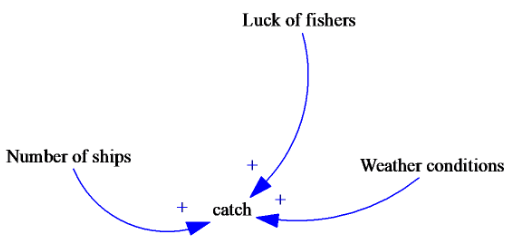
\includegraphics{figures/linearThinking.png}
\caption{Linear Thinking}
\end{figure}

\hypertarget{feedback-thinking}{%
\subsection{Feedback Thinking}\label{feedback-thinking}}

\begin{figure}
\centering
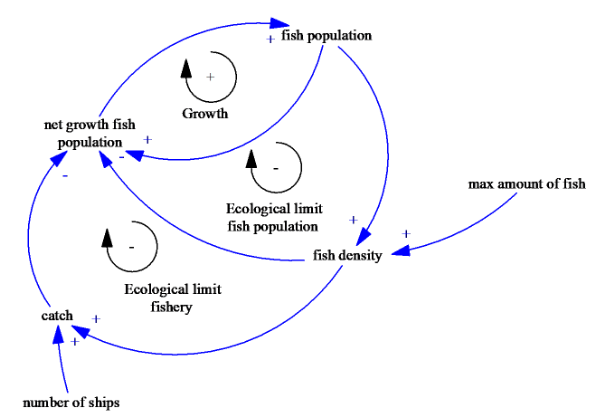
\includegraphics{figures/feedbackThinking.png}
\caption{Feedback Thinking}
\end{figure}

We derive the essential dynamics from the mechanisms within the system
boundaries.

With feedback the catch will decrease due to multiple boats because the
sea is getting outfished (but I have no idea, I'm from Switzerland). In
linear think such a behaviour would not be possible.

\hypertarget{goals}{%
\subsubsection{Goals}\label{goals}}

\textbf{Understanding, not forecasting}\\
The goal of a system dynamics policy study is understanding the
interactions in a complex system that are conspiring to create a
problem, and understanding the structure and dynamic implications of
policy changes intended to improve the system's behaviour (Richardson
1991: 164)\\
\textbf{Modeling for learning}\\
Therefore, the primary goal is not to build the model of the system, but
rather to get a group engaged in building a system dynamics model of a
problem in order to see to what extent this process might be helpful to
increase problem understanding and to devise courses of action to which
team members feel committed (Vennix 1996: 3, emphasised in the
original)'.

\hypertarget{accumulation}{%
\section{Accumulation}\label{accumulation}}

\emph{Understanding accumulation is fundamental to understanding system
behaviour.}

The development of an entity of time is defined by the hydraulic
metaphor, and the equivalent mathematical equation, below.

With the stock-and-Flow-Diagram, you show the inflow, the outflow and
the current stock. 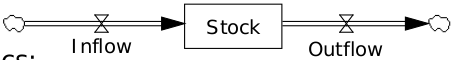
\includegraphics{figures/stocknflow.png}

\emph{A stock takes time to change, because flows take time to flow.
That's a vital point, a key to understanding why systems behave as they
do.}

Stocks: - are state values, the ``memory'' of a system - Need an initial
value - Only change via In-and Outflows - Value does not change <->
Inflow= Outflow - Value increases <-> Inflow\textgreater{} Outflow - Value
decreases <-> Inflow\textless{} Outflow - have units such as liter, CHF,
meter

\hypertarget{difference-between-casual-loop-diagram-and-stock-and-flow-diagram}{%
\subsection{Difference Between Casual Loop Diagram and Stock-and-Flow
Diagram}\label{difference-between-casual-loop-diagram-and-stock-and-flow-diagram}}

\begin{figure}
\centering
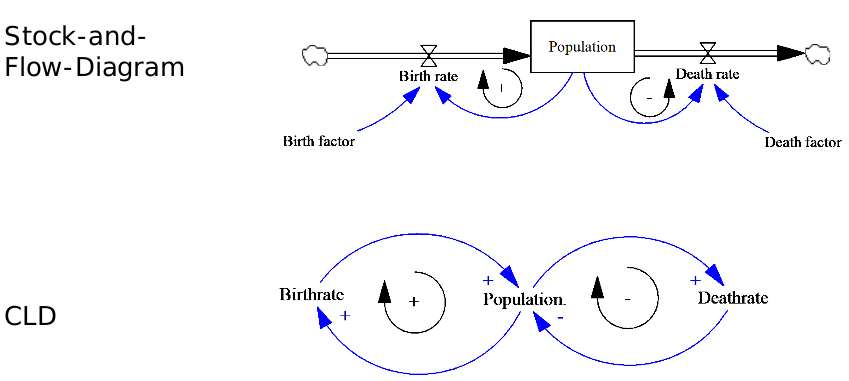
\includegraphics{figures/cldVsStockFlow.png}
\caption{Differences}
\end{figure}

\hypertarget{cld-benefits}{%
\subsubsection{CLD Benefits}\label{cld-benefits}}

\begin{itemize}
\tightlist
\item
  Create an overview and understand a complex system
\item
  Uncover leverage points
\item
  Reduce the complexitiy in finding potential side-effects and feedback
  from policy interventions
\item
  Identify dependent variables \& potentially conflicting goals
\item
  Improve quality of discussion by precise presentation of the subject
  of matter.
\end{itemize}

\hypertarget{rules-for-good-clds}{%
\subsubsection{Rules for good CLDs}\label{rules-for-good-clds}}

\begin{itemize}
\tightlist
\item
  Variable name : Rule 1-3
\item
  Causal relations: Rule 4 - 9
\item
  Loops: Rule 10 - 11
\item
  Model: Rule 12
\end{itemize}
